\chapter{Transcription Alignment for Highly Fragmentary Historical Manuscripts: The Dead Sea Scrolls}

\section{Abstract}
Most of the Dead Sea Scrolls have now been digitally transcribed and imaged to
very high standards. Our goal is to align the transcriptions with the text
visible in the image, glyph by (often fragmentary) glyph. 
This involves several tasks, normally considered in isolation: 
(A) Baseline segmentation.  
(B) Line polygon extraction.  (C) Automated transcription by handwritten
character recognition, to aid in alignment.  (D) Alignment of the Unicode
characters in a line transcription with the characters in the image of that
line.  The task is frustrated by the degraded nature of the frequently very
small and/or warped fragments with many broken letters, substantially different
allographs, ligatures, and scribal idiosyncrasies.  Furthermore, a great number
of inconsistencies between current cataloguing systems for the data need to be
resolved.  For each task, we apply state-of-the-art machine-learning methods in
addition to more traditional techniques, each presenting significant
difficulties on account of the poor state of most fragments' preservation.   

We have built ground-truth datasets and have managed to achieve good results
with well-preserved fragments by leveraging heavily augmented transfer learning
from prior work with medieval manuscripts.

\epigraph{Dedicated to the late Yaacov Choueka (1936--2020), pioneer in
natural language processing and historical manuscript analysis. May his memory
be blessed.}{}
\section{Background}

The Dead Sea Scrolls (dated to the turn of the Common Era) are of enormous
historical significance.  They are the oldest witnesses of the biblical books
and contain a treasure-trove of texts that have shed light on ancient Judaism
shortly before and up into the time of Jesus and Paul.  Their study continues
to revolutionize our understanding of the evolution of Judaism and the
emergence of Christianity.  Unfortunately, the scrolls, or rather the
fragments, were discovered in the 20th century \textsc{ce} in very poor
condition, having deteriorated over the millennia.  Few are large enough to
contain even several columns.\footnote{For an example of a fragment from the
book of Leviticus, see Fig.~\ref{fig:ms}.} The vast majority show only a low
number of words or even just a few letters, many of which are only partially
visible.  Over the past decades, all texts have been painstakingly transcribed
by scholars.  The texts are so fragmentary that the editions have developed
systems to distinguish between certain, probable, possible, and entirely
restored letters.  Taking only the certain and probable letters into
consideration, the average fragment contains about 53 letters.  However, the
few scrolls with almost entirely preserved columns skew the mean as the median
fragment contains only 13 letters.  The extant fragments have recently been
digitized by the Israel Antiquities Authority (IAA) using state-of-the-art
multispectral
imaging.\footnote{\url{https://www.deadseascrolls.org.il/explore-the-archive}}
Older infrared images, photographed under the auspices of the Palestine
Archaeological Museum (PAM) in the 1950s, are likewise available in
retrodigitized form.

Virtually all the texts have been transcribed and most appeared in the
\textit{Discoveries in the Judaean Desert (DJD)}
series,\footnote{\url{http://orion.mscc.huji.ac.il/resources/djd.shtml}} in
Qimron's
edition,\footnote{\url{https://zenodo.org/record/3737950\#.XoXRs6gzaiM}} and in
the \textit{Qumran-Wörterbuch (QWB)} database of the Akademie der
Wissenschaften zu
Göttingen.\footnote{\url{http://www.qwb.adw-goettingen.gwdg.de}} As the only
resource that was truly computationally accessible at the start of this
project, we based our work on the latter.  See Fig.~\ref{fig:trans}.

\section{Introduction}

Our objective is to develop an automated system to align transcriptions of the
texts of the scroll fragments with the visible glyphs on the scroll images on
the individual glyph level.  Achieving this end requires isolating the
fragments in an image from the background so that its text lines can be
identified.  The alignment of transcribed letters with glyphs appearing in the
images of each line is then aided by recognizing at least some of the letters
and spaces.  The processes developed here are closely related to the ongoing
work of several major research projects.

The DIP \textit{Scripta Qumranica
Electronica}\footnote{\url{http://qumranica.org}} (SQE) 
%is a DIP-supported project that 
aims to provide the scholarly community with an open source web-based portal
for the purposes of material analysis of the  scrolls.  It combines the
high-resolution image database of the IAA with the QWB lexical database.  A
feature-rich suite of digital tools and computational methods are brought
together to create an infrastructure for the production of digital editions
\cite{SQE}. %Cite the Haifa article in EBR also 

The University of Groningen 
%(ERC-funded) 
project, \textit{The Hands that Wrote the
Bible},\footnote{\url{https://cordis.europa.eu/project/id/640497}} is dedicated
to investigating the paleography of the Dead Sea Scrolls.  It has so far
produced a benchmark study in writer identification \cite {DhaliEtAl2017} and
advances in dating \cite{DhaliEtAl2020dating} and in binarization techniques of
these manuscripts \cite{DhaliEtAl2019}.

Nearly all of the Dead Sea Scrolls are written in Hebrew letters on animal
skin, i.e.\@ parchment, but phenomenologically they are very close to papyrus,
which is mostly from ancient Egypt and written in Greek.  The University of
Basel 
project, \textit{Reuniting fragments, identifying scribes and characterizing
scripts: the Digital palaeography of Greek and Coptic papyri},%
\footnote{\url{https://altegeschichte.philhist.unibas.ch/de/digpaleo}}
organized a binarization competition \cite{Pratikakis2019} and published a
dataset on writer identification \cite{Mohammed2019b}.  In addition, the
Wuerzburg-Heidelberg-Paris project, PapyroLogos, works on text-image alignment
of literary and documentary Greek papyri \cite{KiesslingStoekl2019}.

Other major projects on Hebrew manuscript material include the 
Friedberg Genizah Project, which digitized hundreds of thousands of fragments
of medieval manuscripts, mostly in Hebrew, Judeo-Arabic, and Aramaic
\cite{FGP}.\footnote{\url{https://fgp.genizah.org}} State-of-the-art
computational tools were developed for segmentation \cite{Catalog}, paleography
\cite{Paleo}, matching fragments by handwriting and codicological features
\cite{Join}, and word spotting \cite{Spot}. 

The Sofer Mahir project strives to create open source transcriptions of ca.\@
6000 pages of 18 substantial manuscripts of the earliest Rabbinic literature
(Mishnah, Tosefta and Midreshei
Halakhah).\footnote{\url{https://sofermahir.hypotheses.org}} In the Tikkoun
Sofrim project,  crowdsourcing and machine learning is used to correct errors
in the automatic transcriptions of manuscripts of medieval exegetical
literature
\cite{Kuflik2019}.\footnote{\url{https://tikkunsofrim.hypotheses.org}}

\begin{figure}[t] \centering
	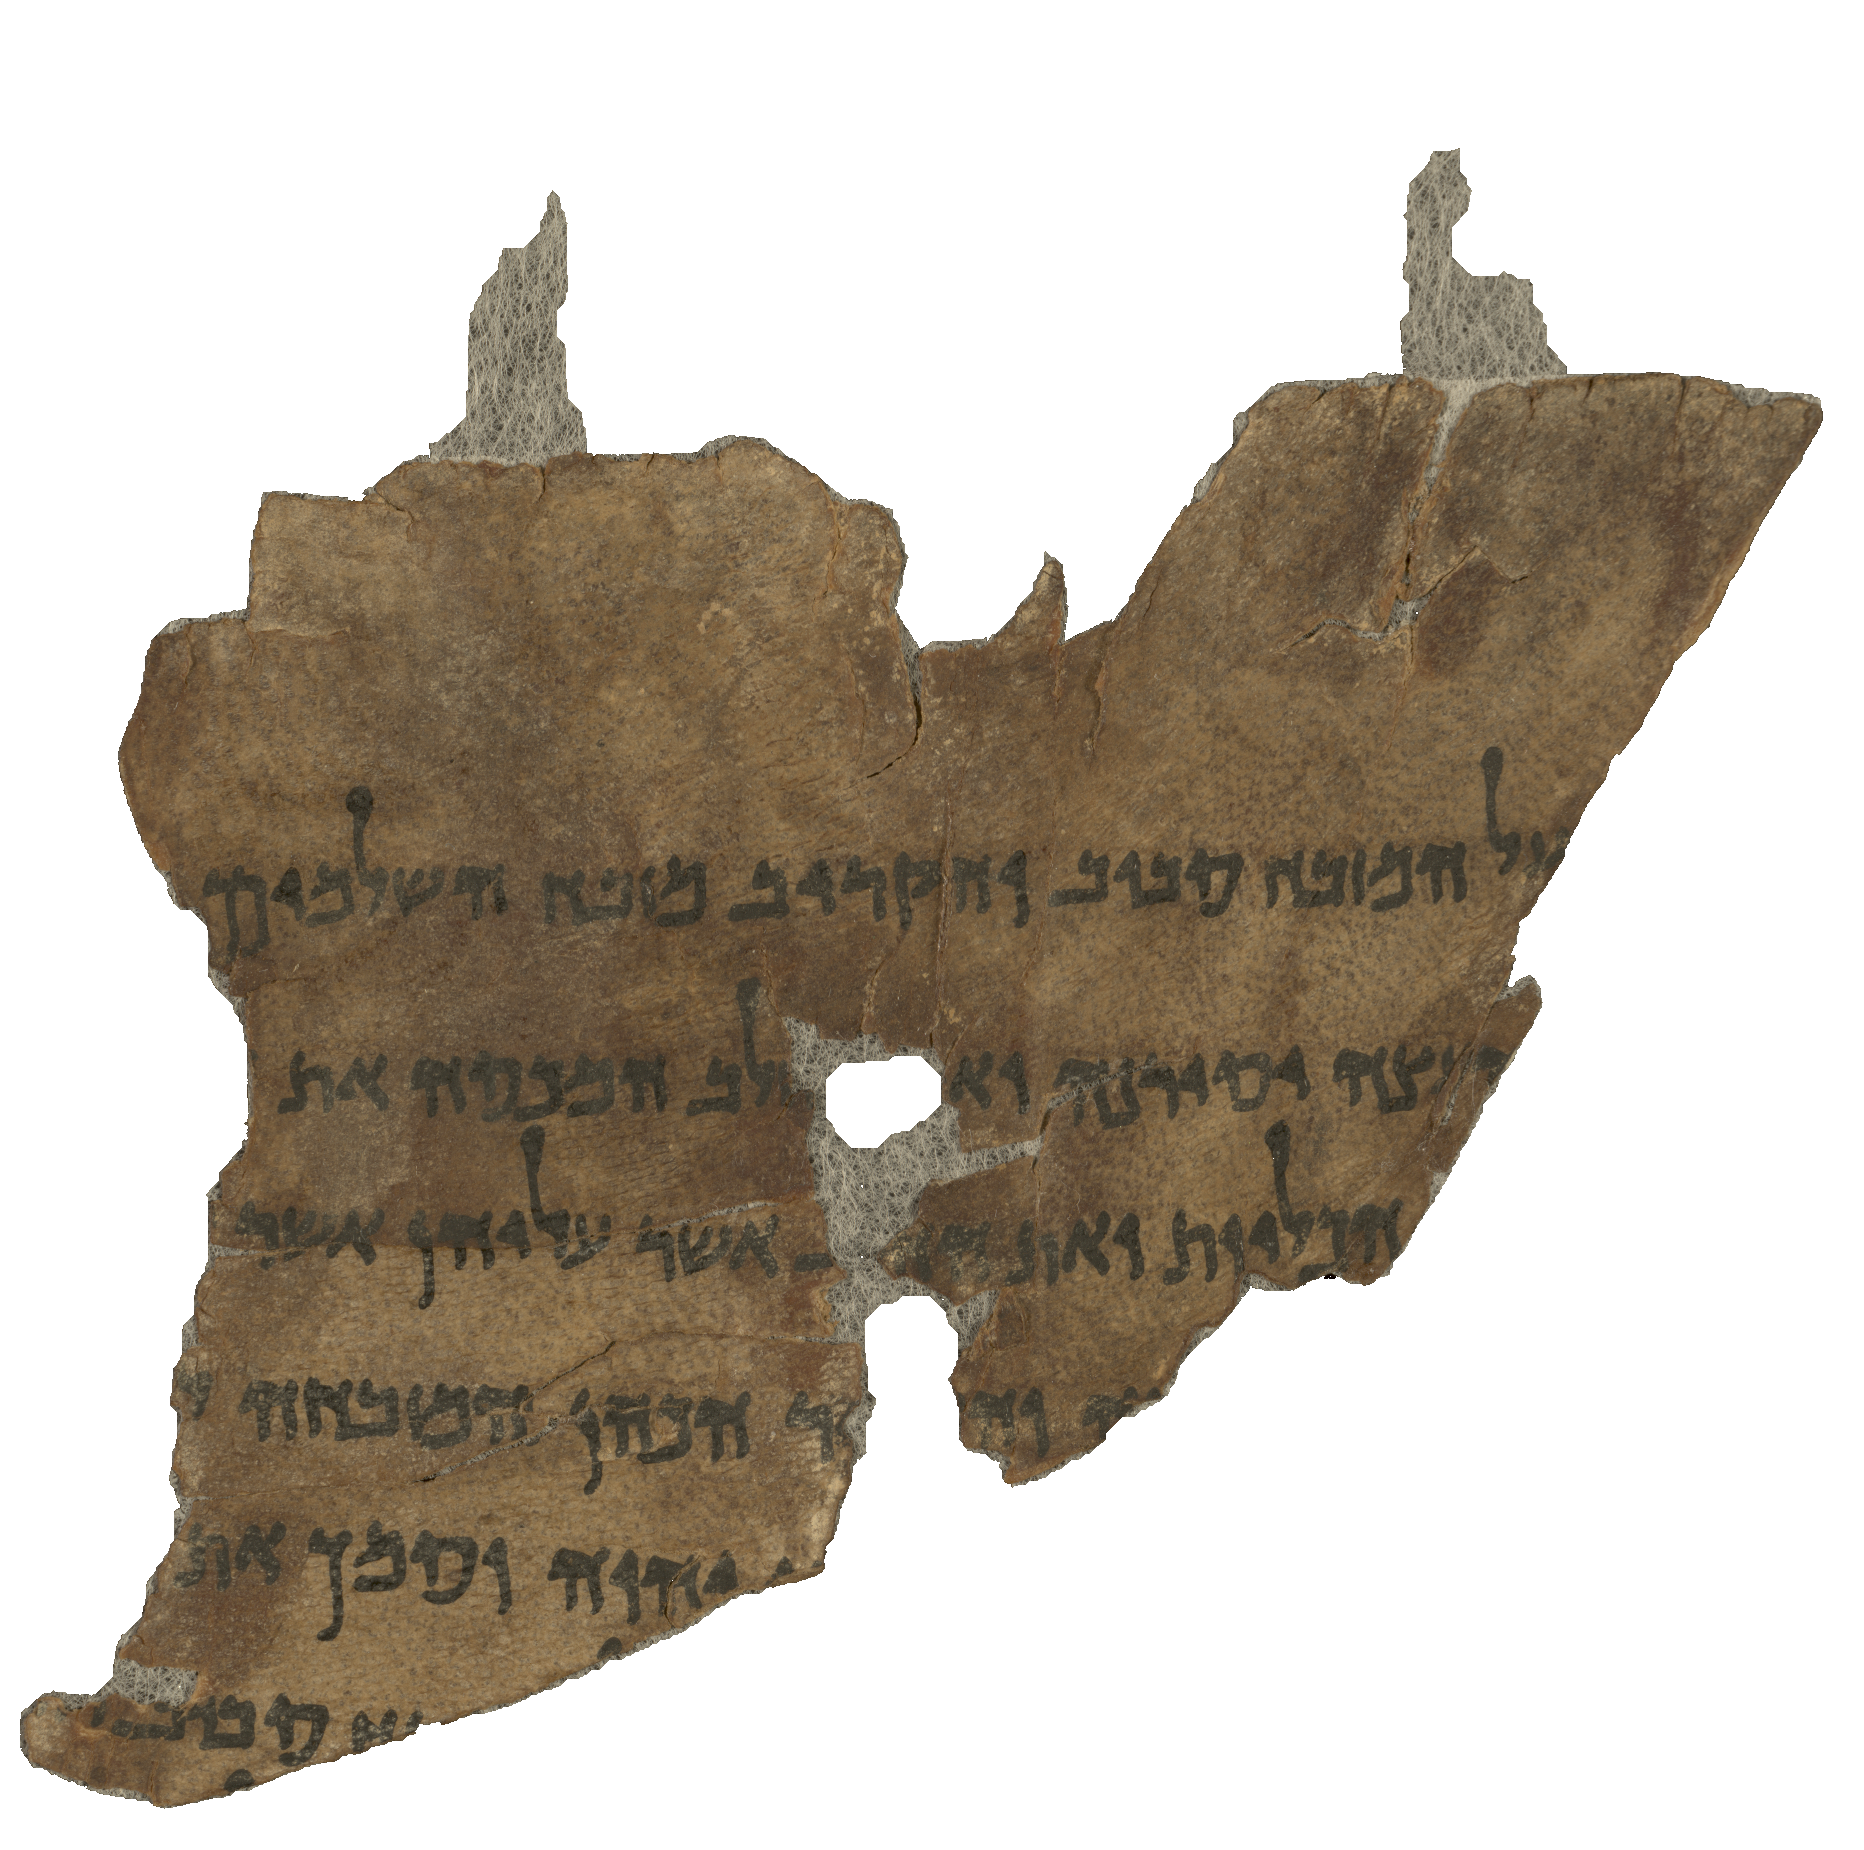
\includegraphics[width=.5\textwidth]{images/ms.png}
	\caption{Manuscript fragment (Leviticus 3) after imperfect foreground
	segmentation. All images of fragments are courtesy of the Leon Levy
	Dead Sea Scrolls Digital Library, Israel Antiquities Authority. Photos:
	Shai Halevi.\label{fig:ms}}
\end{figure}

\begin{figure}[t] \centering
	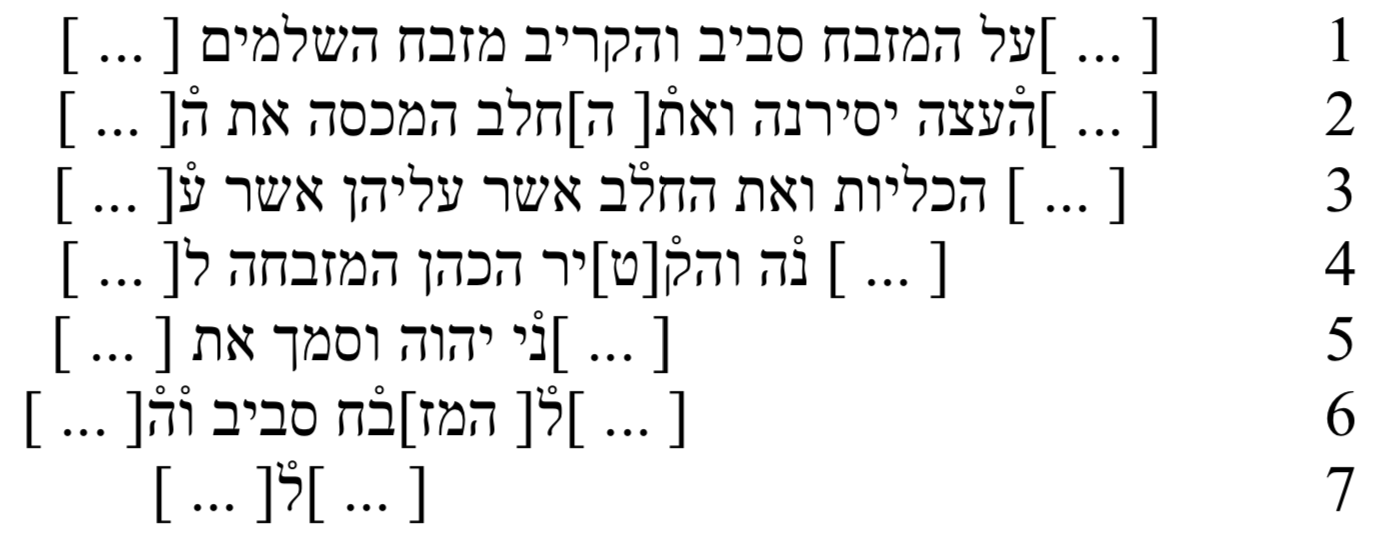
\includegraphics[width=.7\textwidth]{images/4Q24_f8.png} 
	\caption{Scholarly transcription of the fragment (4Q24 fr. 8) in Fig.}%~\ref{fig:ms}.}
	\label{fig:trans}
\end{figure}

\begin{figure}[t] \centering
	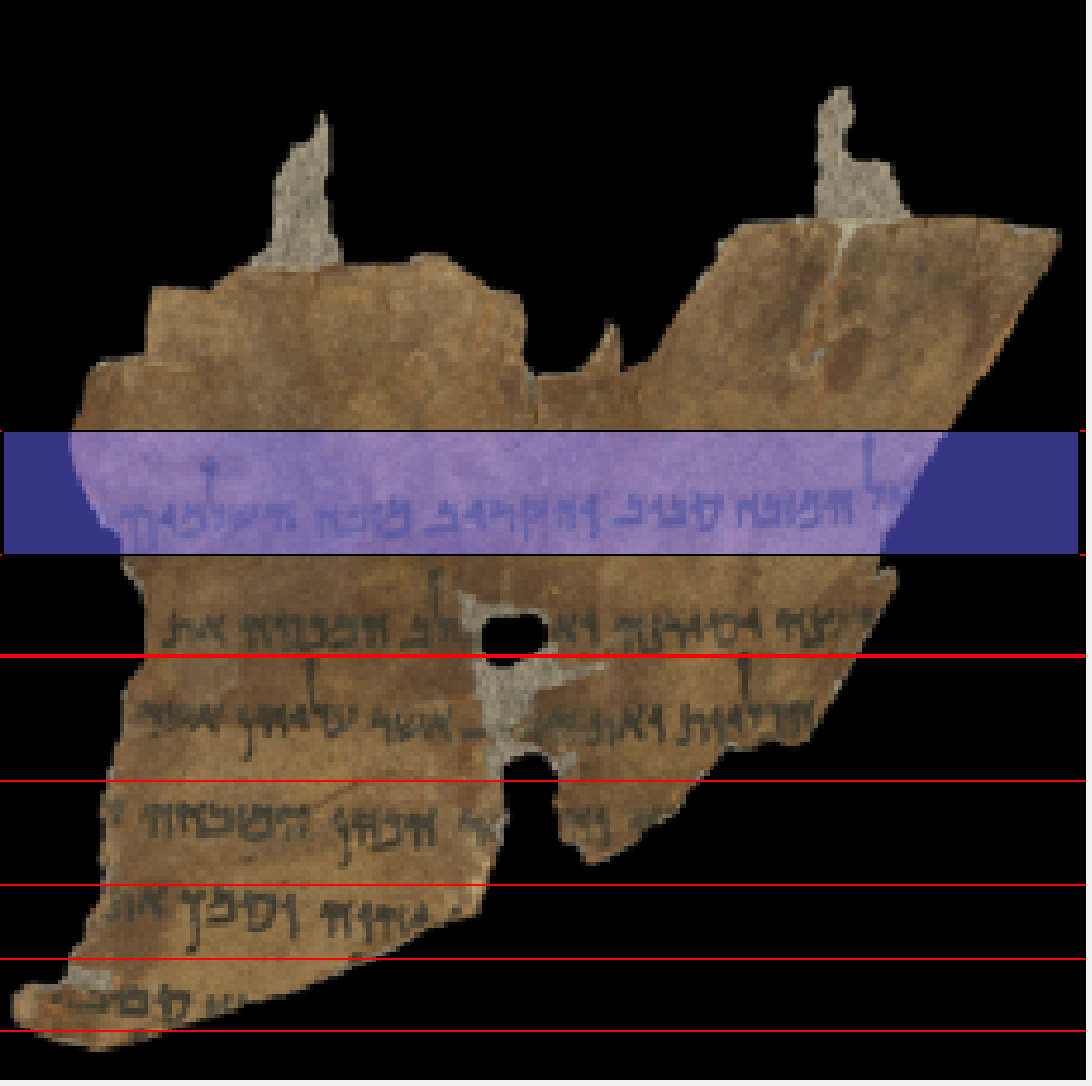
\includegraphics[width=.5\textwidth]{images/lines.png}
	\caption{Line segmentation of the fragment in Fig.}%~\ref{fig:ms}.}
	\label{fig:lines}
\end{figure}

\section{Methods and Related Work}

Different infrastructures allow automatic interaction with historical
manuscripts (a brief overview is given in \cite{KiesslingEtAl2019eScrip}).
Most notable are Transkribus
\cite{Kahle}\footnote{\url{https://transkribus.eu/Transkribus}} and MONK
\cite{schomaker2019lifelong},\footnote{\url{http://www.ai.rug.nl/~lambert/Monk-collections-english.html}}
which are however not open source and, at least in the case of Transkribus also
commercial,\footnote{\url{https://readcoop.eu/transkribus-pricing}} and
therefore much more difficult or even impossible to include in a full treatment
pipeline.  The only cutting edge and fully open-source infrastructure for
historical document analysis we know of is eScriptorium \cite{escript19}.%
\footnote{\url{https://escripta.hypotheses.org}}
Accordingly, we have made use of its tools and have performed the following
procedures.

\subsection{Line Segmentation} After a long predominance of methods relying on
traditional computer vision approaches to perform text line extraction from
handwritten documents, machine learning based systems have seen wider use
recently
\cite{KiesslingEtAl2019Badam,gruning2018read,fink2018baseline,diem2017cbad,KurarBarakat2018}.
The majority of these methods utilize combinations of CNNs and LSTMs. Still,
traditional methods from computer vision can have advantages for certain tasks
or types of manuscripts \cite{Viral,Seuret,StoeklLapinForthcoming}.  We tested
several hand-crafted line segmentation algorithms without success, settling on
a trainable method described in \cite{KiesslingEtAl2019Badam,
KiesslingStoekl2019}, as implemented in kraken \cite{Kraken} and eScriptorium.
Layout analysis is independent of binarization and works very well even on
highly fragmentary and damaged material (such as the Dead Sea Scrolls and the
Genizah); see Fig.\ref{fig:baselinesegm}.

\begin{figure}[t]
	\subfloat{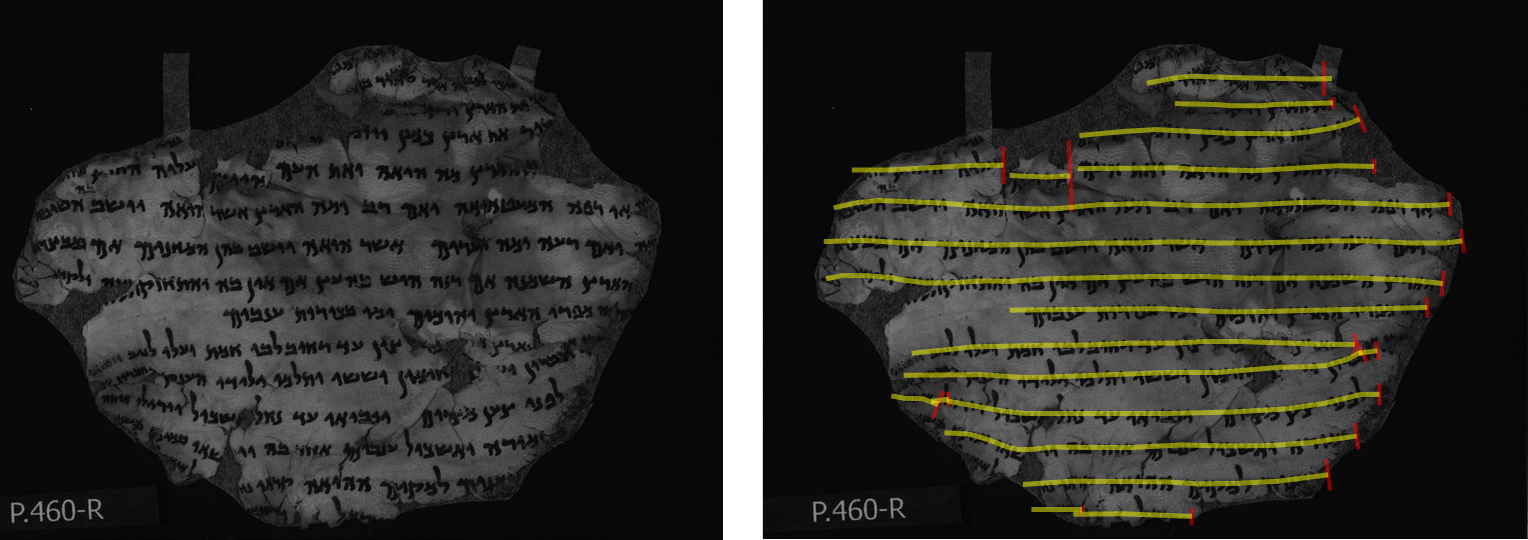
\includegraphics[width=1\columnwidth]{images/528b.PNG}}\\ 

\subfloat{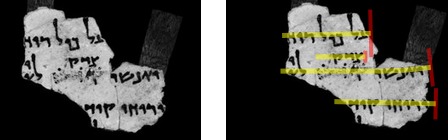
\includegraphics[width=1\columnwidth]{images/584_cropped.png}}
	\caption{Automatic segmentation result (left without, right with
	baselines marked in yellow and an additional right vertical bar marking
	the beginning) of a large (top) medium (bottom) size fragment.}
\vspace*{-5mm} \label{fig:baselinesegm} \end{figure}

\subsection{Automated Transcription}

In line with the state of the art in text image classification we utilize a
hybrid CNN-RNN trained in a supervised manner to classify sequences of
characters on whole text lines using the connectionist temporal classification
loss \cite{graves2006connectionist}. The kraken OCR engine's recognizer with
default parameters is used instead of a custom implementation.

Due to the challenging nature of the material such as high script variability
and extensive degradation, even the best modern OCR engines perform quite
poorly ($<$ 90\% CER). While unsuitable for close reading, even poor-quality
OCR output can be serviceable for novel applications like intertextuality and
search.  In contrast to exact search as implemented in standard search engines,
which yields very limited results, approximate search can be both applied to
finding individual phrases \cite{approx,Wiener} and to matching against an
existing corpus \cite{Zh}.  Our method for text identification based on
approximate search is detailed in Section \ref{sec:id}.

\subsection{Transcription Alignment}

Early work on aligning OCR text with ground truth is presented in \cite{Hobby}.
More recent work includes
\cite{DBLP:conf/jcdl/FengM06,DBLP:conf/icdar/YalnizM11,DBLP:conf/icdar/0002FFB11,OFTA,Leydier2014alignment,dense,Leydier2016alignment,Boillet2019}.
We experimented with (a) optical SIFT-flow \cite{OFTA}, (b) alignment with OCR
results -- by means of minimal edit distance, and (c) a combination -- using
anchors obtained from the OCR to constrain the optical flow.

For optical SIFT-flow we first render the known Unicode transcription as a line
image in a manner and font that is similar to the manuscript.  Next, a visual
alignment is made between the synthetic transcription image and the original
manuscript image by the SIFT flow image matching algorithm introduced in
\cite{liu2011sift}.  Since we have information regarding the letter boundaries
in the rendered image, these boundaries translated into the manuscript image by
the retrieved optical alignment result in an approximation of the letter
boundaries in the manuscript image, thus resulting in a glyph alignment.  To
enhance the visual alignment, we may use previously discovered correspondences
between the rendered image and the manuscript image, which we call anchors for
the optical alignment, in order to align the images more precisely.  These
anchors might be gained, for instance, from character or inter-word bounding
boxes found by the OCR algorithm. 

In the OCR based method, we first train a recognition model on the known
transcription-line pairs with kraken until the system overfits the data.  We
then apply the same model on the data on which it was trained.  We can
extrapolate the approximate $x$-coordinate of the character boundaries based on
the highest activation time-step returned by the system for a given character.
The $y$ coordinates can be estimated from the line polygon.

\section{Experimental Results}

\subsection{Corpus Sample}\label{sec:seg}

The base data for the following analyses are the images from the Leon Levy Dead
Sea Scrolls Digital Library and the text transcription of the Qumran Wörterbuch
Project.  These projects made use of two different and only sometimes
overlapping cataloguing systems, which complicated the correlation of image to
a specific set of transcriptions.  After aligning the two systems by applying
various adaptive rules for entry matching and some manually specified
correlations, images were selected for which reliable matches to the textual
transcriptions were available.\footnote{The results of the merging of these two
catalogues can be accessed through the SQE web API
\url{https://api.qumranica.org/swagger}.}

For many reasons, the catalogue remains perfectible.  The definition of what is
a fragment is not straightforward and the fragments continued to ``live" and
change after their publication.  In the new photographs, a fragment is a
physical unit that can be lifted in one piece from its archival plate.
However, such a unit may constitute several different fragments in the editions
that have been joined, for instance, with Japanese rice paper in a later
conservation process.  In other cases, the editor gave a single identifier to
what constitute several distinct physical units depicted on distinct images.
Other fragments, still in one piece in the edition, have since broken up or
disintegrated into several pieces.  Some images in the image database are
identified as representing a specific fragment while in fact the current
fragment only contains a fraction of the published text.  Several
identifications were incorrect, and a few imaged fragments were not identified
at all.  Therefore, we had to verify the identification of each image with its
corresponding transcription from the QWB database.

\subsection{Line Segmentation}\label{sec:lseg}

As a first step, we transfer-learned a new baseline segmentation model on top
of models trained initially on medieval manuscripts and Greek papyri.  We
bootstrapped the training material following a common procedure:  Firstly, we
manually annotated 100 images of Qumran fragments, used them as training
material, and afterwards applied the results to 300 more images of Qumran
fragments.  We then manually corrected the automatic results in the
eScriptorium web interface and used that larger corpus to train another model
to apply to ca.\@ 500 more images.  The ergonomic interface of eScriptorium
makes this usually cumbersome process very easy.  While manually annotating the
baselines of an image from scratch takes approximately 90 seconds, the average
manual correction time for an automatically segmented image is less than 30
seconds for the first stage and less than 15 for the second stage.  However,
depending on the complexity of the layout, the time needed for an image can
differ markedly.  Many images require few or no corrections.  See
Fig.~\ref{fig:alignment_result} for an example.

Some fragments have been imaged at a rotation angle other than upright.
Consequently, we determine the correct reading order based on the median
principal writing angle of the baselines, taking into consideration the writing
direction.  In the near future, we will add the new kraken and escriptorium
feature for automatic segmentation of regions to the pipeline to improve the
results for multi-column fragments, especially regarding the reading
order\cite{KiesslingICFHR2020}. 

\subsection{Automated Transcription}\label{sec:trans}\label{sec:id}

In a second step, we extracted textual data from the QWB database and matched
it linewise to the segmented lines on the images.  We retained only fragments
written in Judean square script leaving out any fragment written in
paleo-Hebrew, Cryptic C, Greek, or Nabatean.  Still the hands of the fragments
vary widely in register, formality, and period and represent many different
scribal habits.  The dates the scrolls were written could vary by 300 years in
a very ``hot" period, that is, a period with massive changes in ductus
according to local schools after the disintegration of the relatively unified
Imperial writing system of the Persian Empire. %There may have been just as
much variation in the Persian Empire (see the 1966 Chicago dissertation of
DAVID WALTER NASGOWITZ).  We discarded all letters marked as restored or as
merely possible readings, keeping only the probable and certain instances.  Due
to the aforementioned complications inherent to the fragments, editions, and
the database, the ``zipping'' together of the image and the textual data is not
a trivial process.  Therefore, the rough OCR of the extant text in the next
step, provided a welcome check, (1) whether the identification of the fragment
image with the corresponding text was correct, (2) whether the fragment was
still complete, and/or (3) whether it had been joined with other fragments.

\begin{figure}[t]%[width=1\columnwidth]
	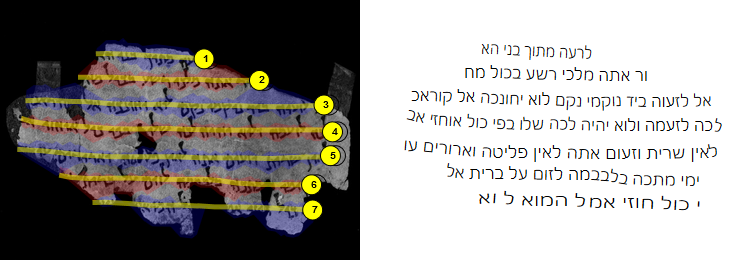
\includegraphics[width=1\columnwidth]{images/40b.PNG}
	\caption{Imageline to textline alignment result as displayed in
	eScriptorium. Baselines are depicted in yellow, boundary polygons in
	alternating red and blue.} \vspace*{-5mm} \label{fig:alignment_result}
\end{figure}

The third step consisted of training a transcription model on the selected
ground truth with a 90/10 training/testing split on the grayscale images
(without binarization).  Discarding misidentified items and fragments in other
scripts, the final training material comprised 33075 characters on 2474 lines
from 440 images.  The testing material read 3403 characters on 247 lines from
44 images.

On the average, we can count 5--6 lines and ca.\@ 75 characters (including
spaces) per fragment.  These are thus relatively large fragments.
 %[1,120,0,1 Cr3,13,32 Do0.1,2 Mp2,2 Cr3,13,32 Do0.1,2 Mp2,2 Cr3,9,64 Do0.1,2
%Mp2,2 Cr3,9,64 Do0.1,2 S1(1x0)1,3 Lbx200 Do0.1,2 Lbx200 Do.1,2 Lbx200 Do] 
New models were trained on top of the models previously trained on medieval
Hebrew manuscripts.
%with a configuration as Fig.~\ref{fig:tikzpic}.

The best model reached an accuracy of 67.9\%  on the test material after 21
epochs. 
% [1,120,0,1 Cr3,13,32 Do0.1,2 Mp2,2 Cr3,13,32 Do0.1,2 Mp2,2 Cr3,9,64 Do0.1,2
% Mp2,2 Cr3,9,64 Do0.1,2 S1(1x0)1,3 Lbx200 Do0.1,2 Lbx200 Do.1,2 Lbx200 Do]
While this may seem very low, we applied the trained models to fragments
outside of the training and test corpora, and the automatic transcriptions were
extremely convincing for most fragments.  The results are in fact better than
the numbers indicate because frequently the transcriptions include very partial
letters of which sometimes only scant remains are visible, in particular in the
top and the bottom row of fragments, but not only.  Even experts would
typically have to expend significant effort evaluating the best reading
possibilities.
%This difficulty is shown by the fact that the best model achieved only 75.2\%
%on the training material.

In particular, the OCR results are sufficient to identify the fragments.  With
a bag of words approach for identification and with rotations every 90{\degree}
to choose the best angle for recognition, the system was able to identify 22
out of 24 available fragments comprising more than 100 characters. 
%\todo{how many?}
In other words, given the imperfect OCR of each fragment and searching for the
words among all 5756 transcriptions in QWB, the best match was indeed the
actual scholarly transcription of the fragment in question.  The two exceptions
were fragments for which the system preferred a fragment of the same
composition but from a different manuscript.

\subsection{Transcript Alignment}\label{sec:al}


%\begin{figure*}[t]
\begin{figure}[t]

%\centering \begin{subfigure}%{0.48\textwidth}
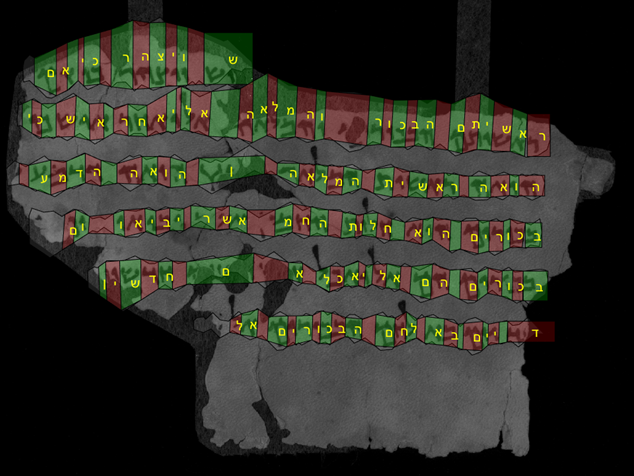
\includegraphics[width=1\columnwidth]{images/P702-Fg010-R-C01-R01-D12092012-T111025-LR924_012_F_rewrite._reordered_with_text._page_cutout.png}
  %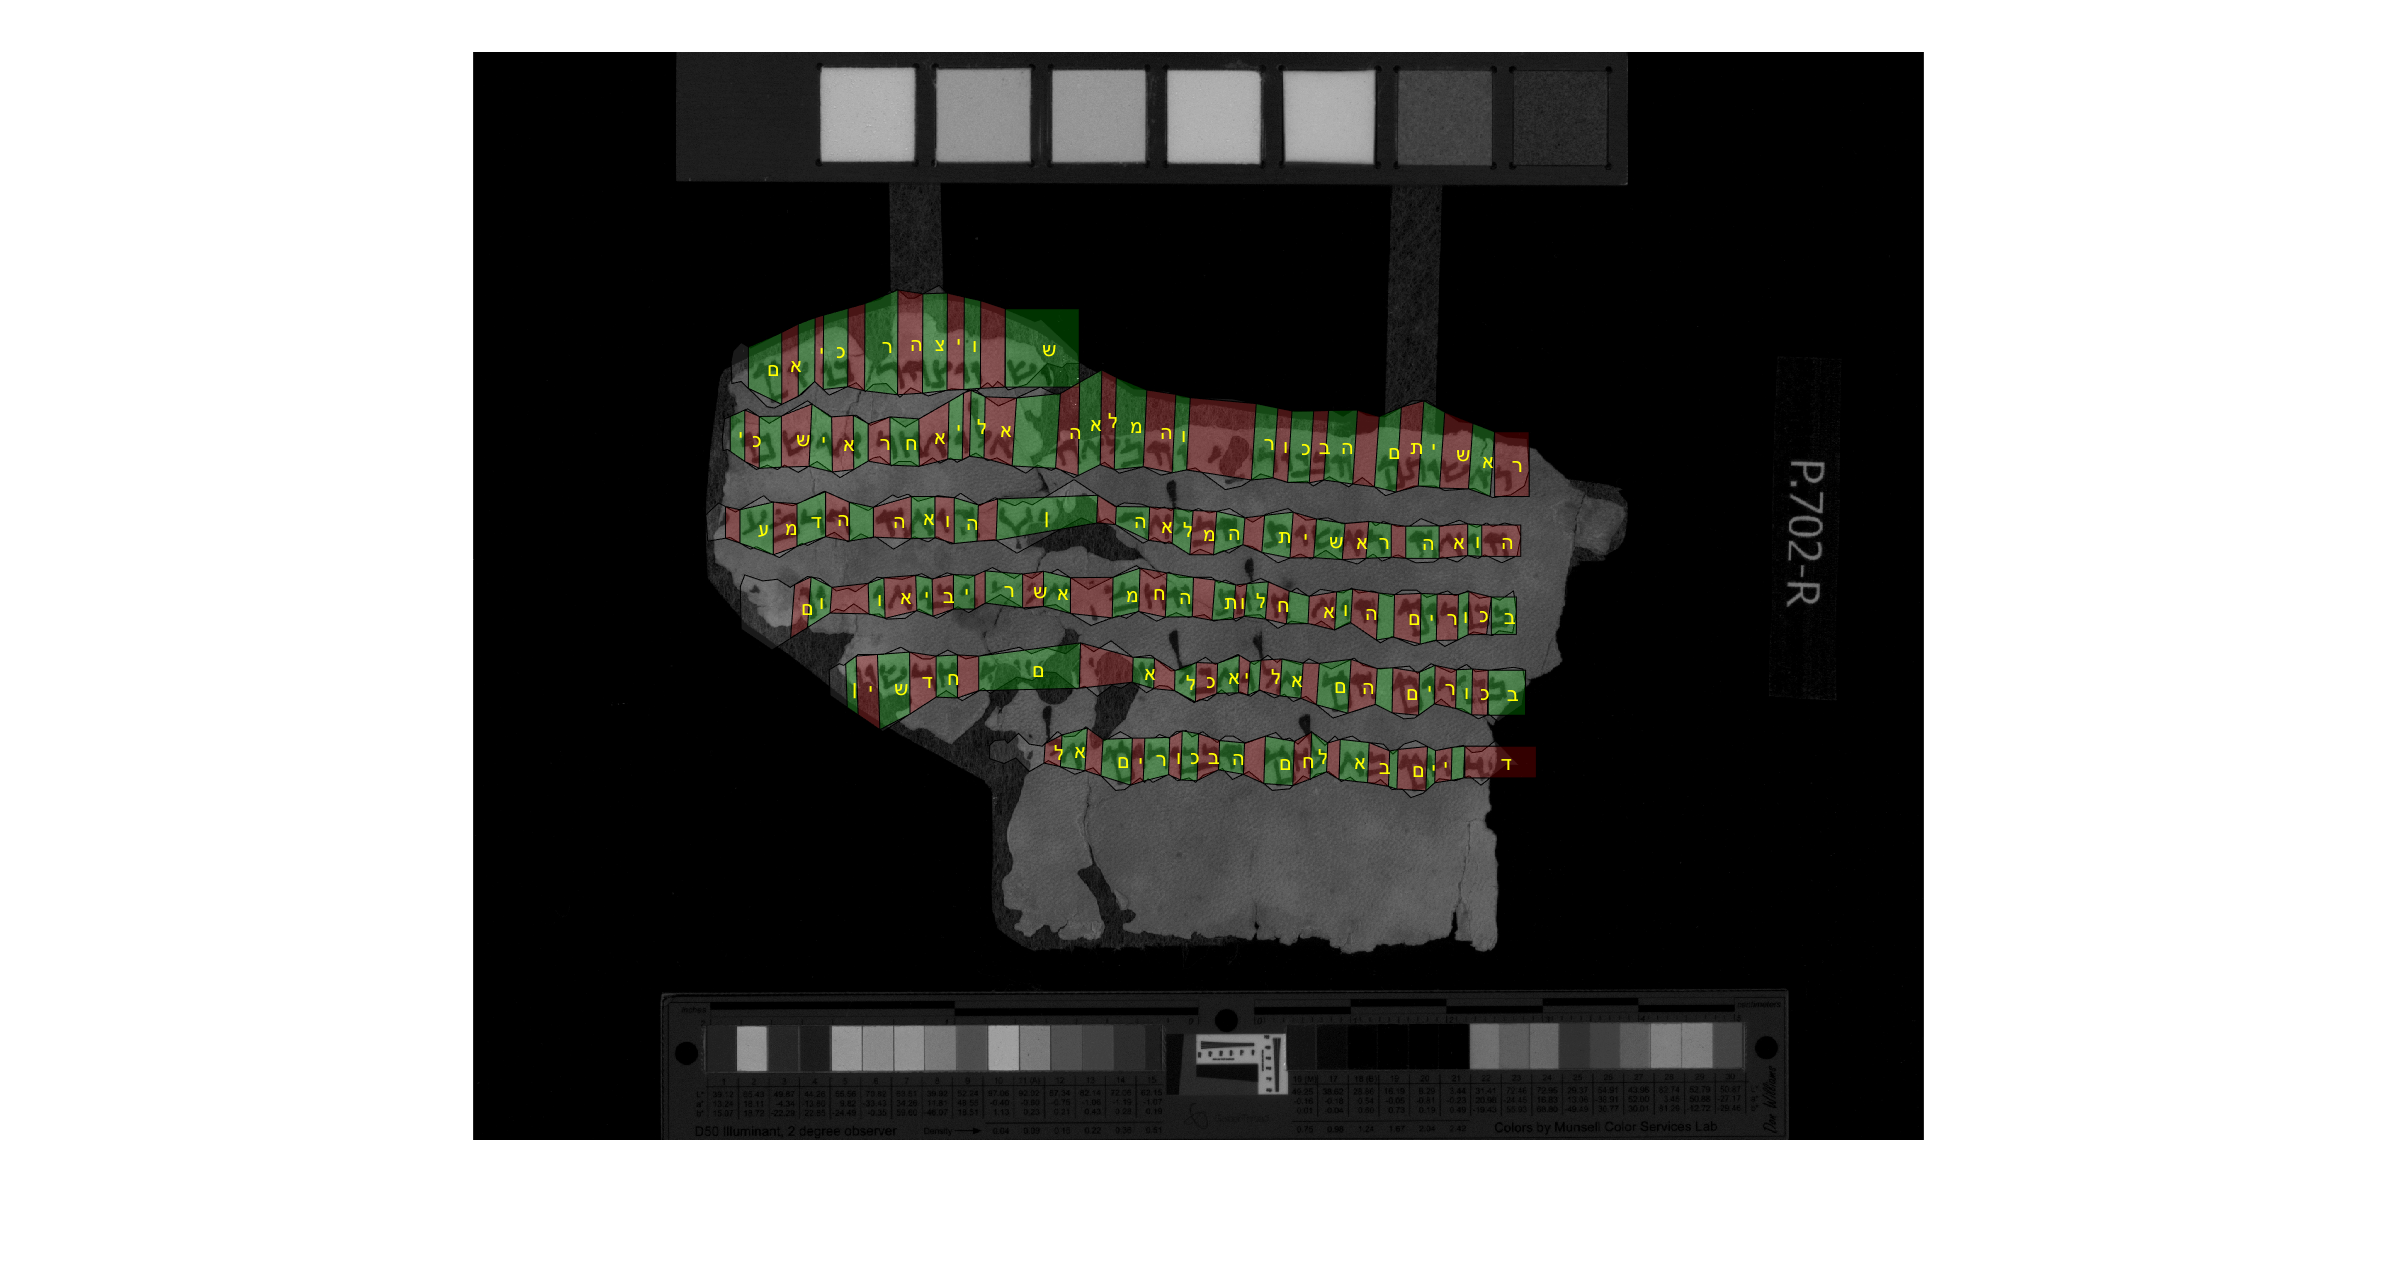
\includegraphics[width=1.0\linewidth]{images/P702-Fg010-R-C01-R01-D12092012-T111025-LR924_012_F_rewrite._reordered_with_text._page.png}
  \label{fig:regularAlignment}
%\end{subfigure} \begin{subfigure}{0.48\textwidth}
  %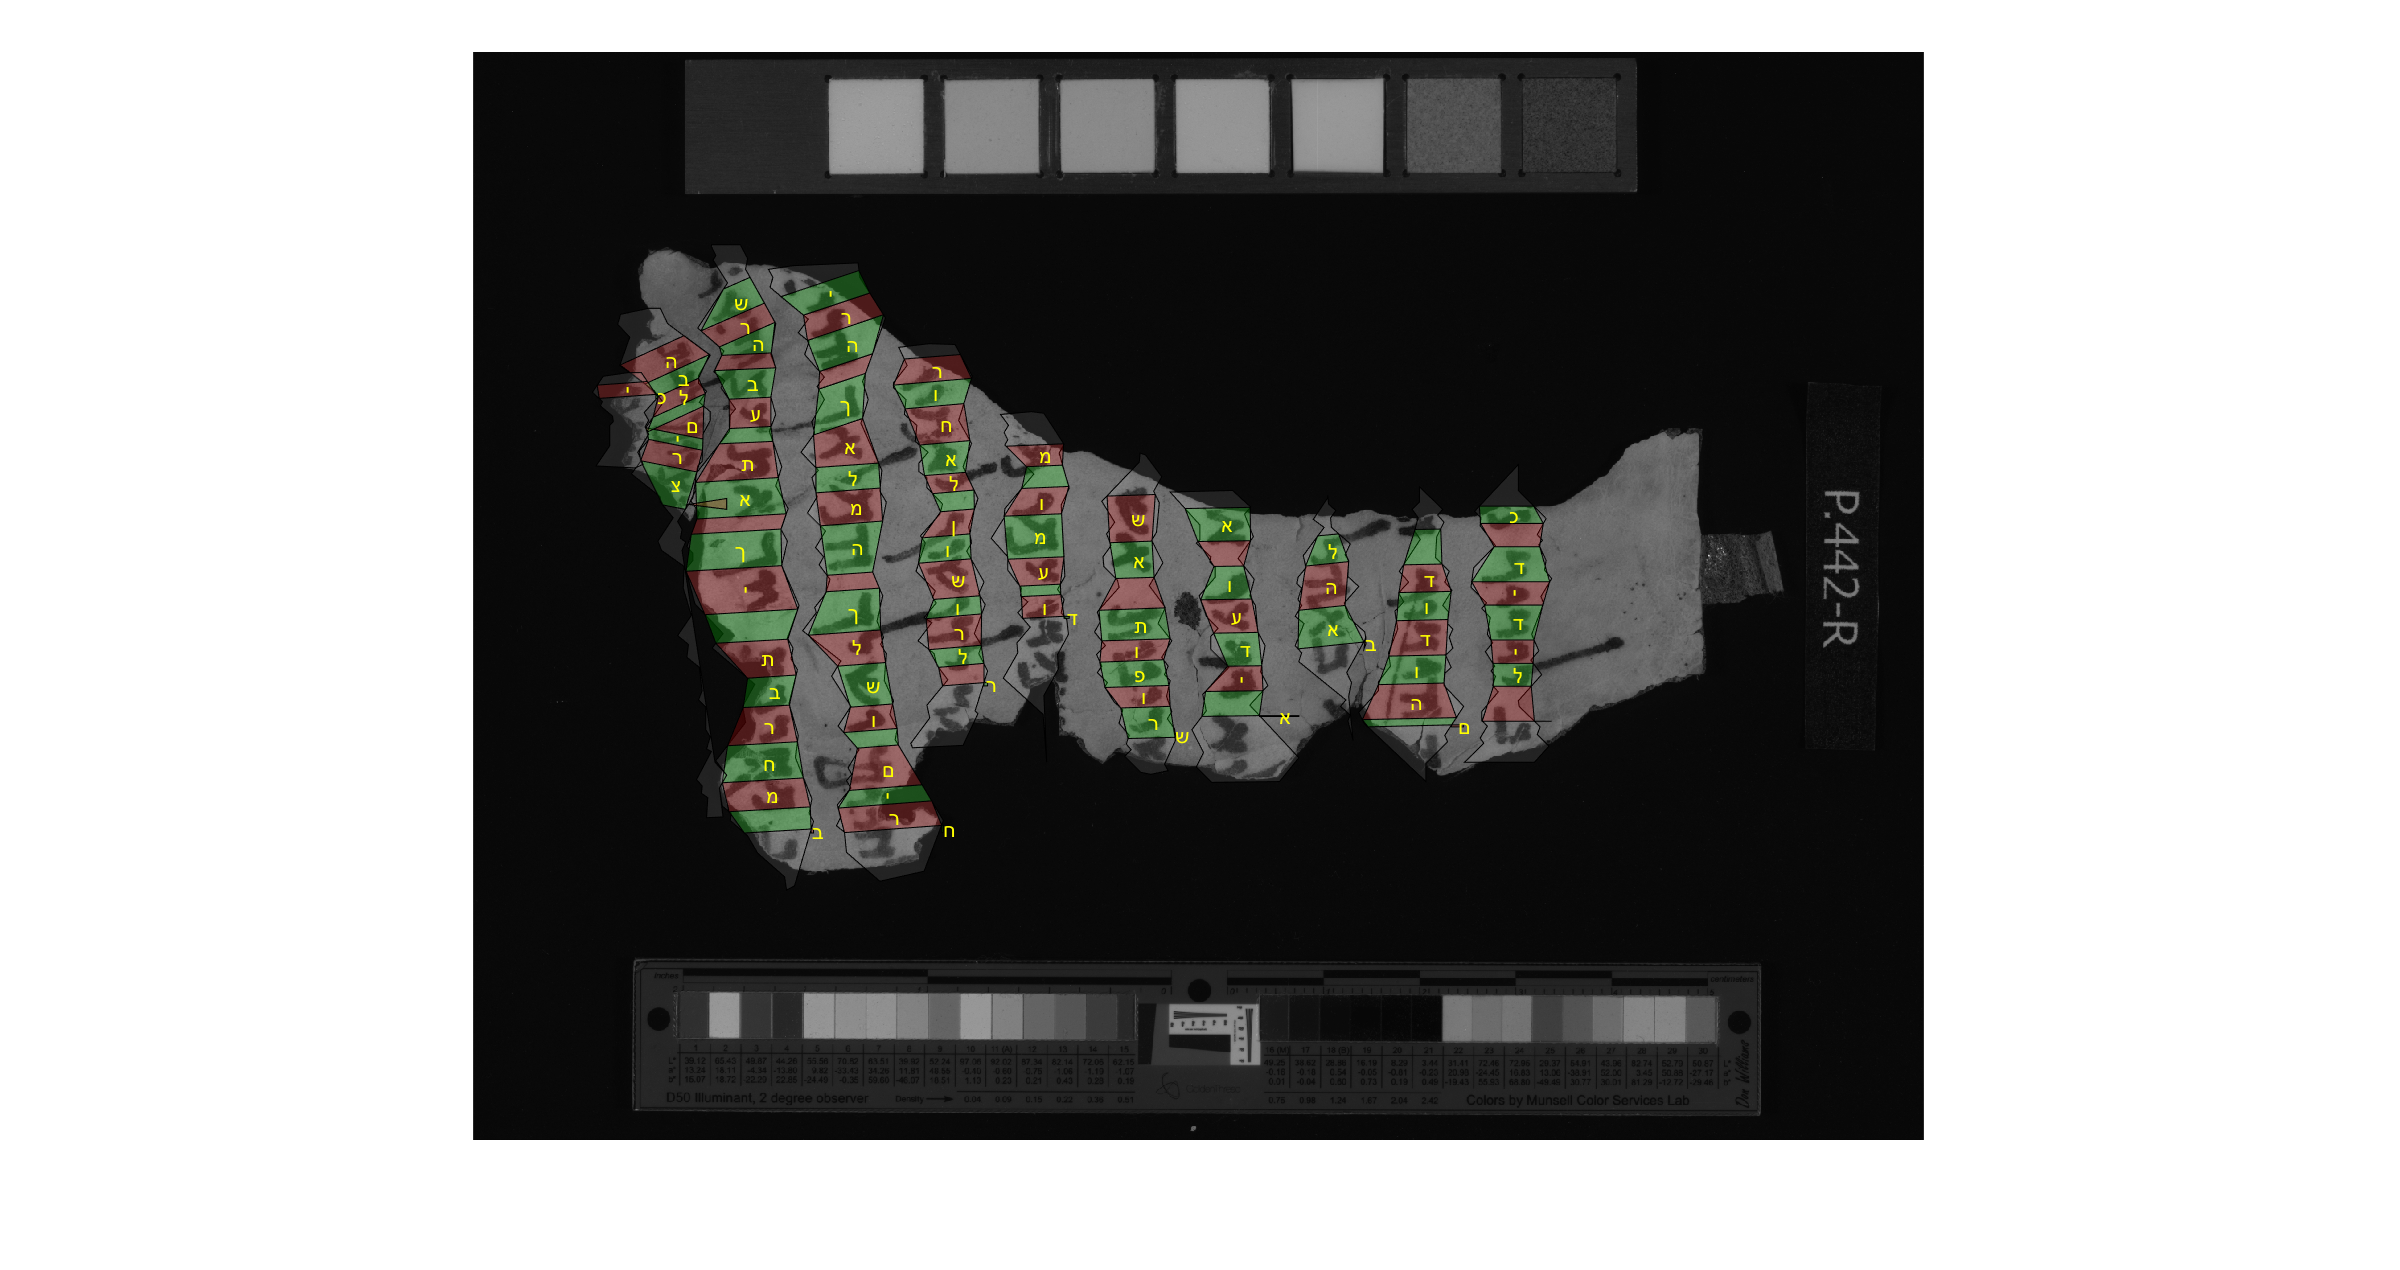
\includegraphics[width=1.0\linewidth]{images/P442-Fg001-R-C01-R01-D01092013-T114646-LR924_012_rewrite._reordered_with_text._page.png}
  %\label{fig:rotatedAlignment} \end{subfigure}
  \vspace*{-5mm} \caption{Aligned glyphs of a whole fragment. Alternating red
	and green polygons indicate areas. Yellow overlay indicates identified
	letter.} \vspace*{-5mm} \label{fig:align}
%\end{figure*}
\end{figure}

\begin{figure*}[t] \centering\ \begin{subfigure}{0.48\textwidth}
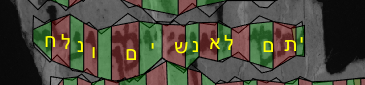
\includegraphics[width=1.0\linewidth]{images/P1094-Fg002-R-line02.PNG}
\label{fig:alignedChars} \end{subfigure} \begin{subfigure}{0.48\textwidth}
	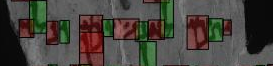
\includegraphics[width=1.0\linewidth]{images/P1094-Fg002-R-line02GT.PNG}
\label{fig:alignedCharsGT} \end{subfigure} \vspace*{-5mm} \caption{Aligned
glyphs of a single line. Left: Automatic alignment with alternating red and
green polygons indicate areas. Yellow overlay indicates identified letter.
Right: Corresponding human annotated ground truth (no interword spaces, no
letter overlay).} \vspace*{-5mm} \label{fig:alignedGlyphs} \end{figure*}

%\begin{figure*}[t] \centering \begin{subfigure}{0.48\textwidth}
%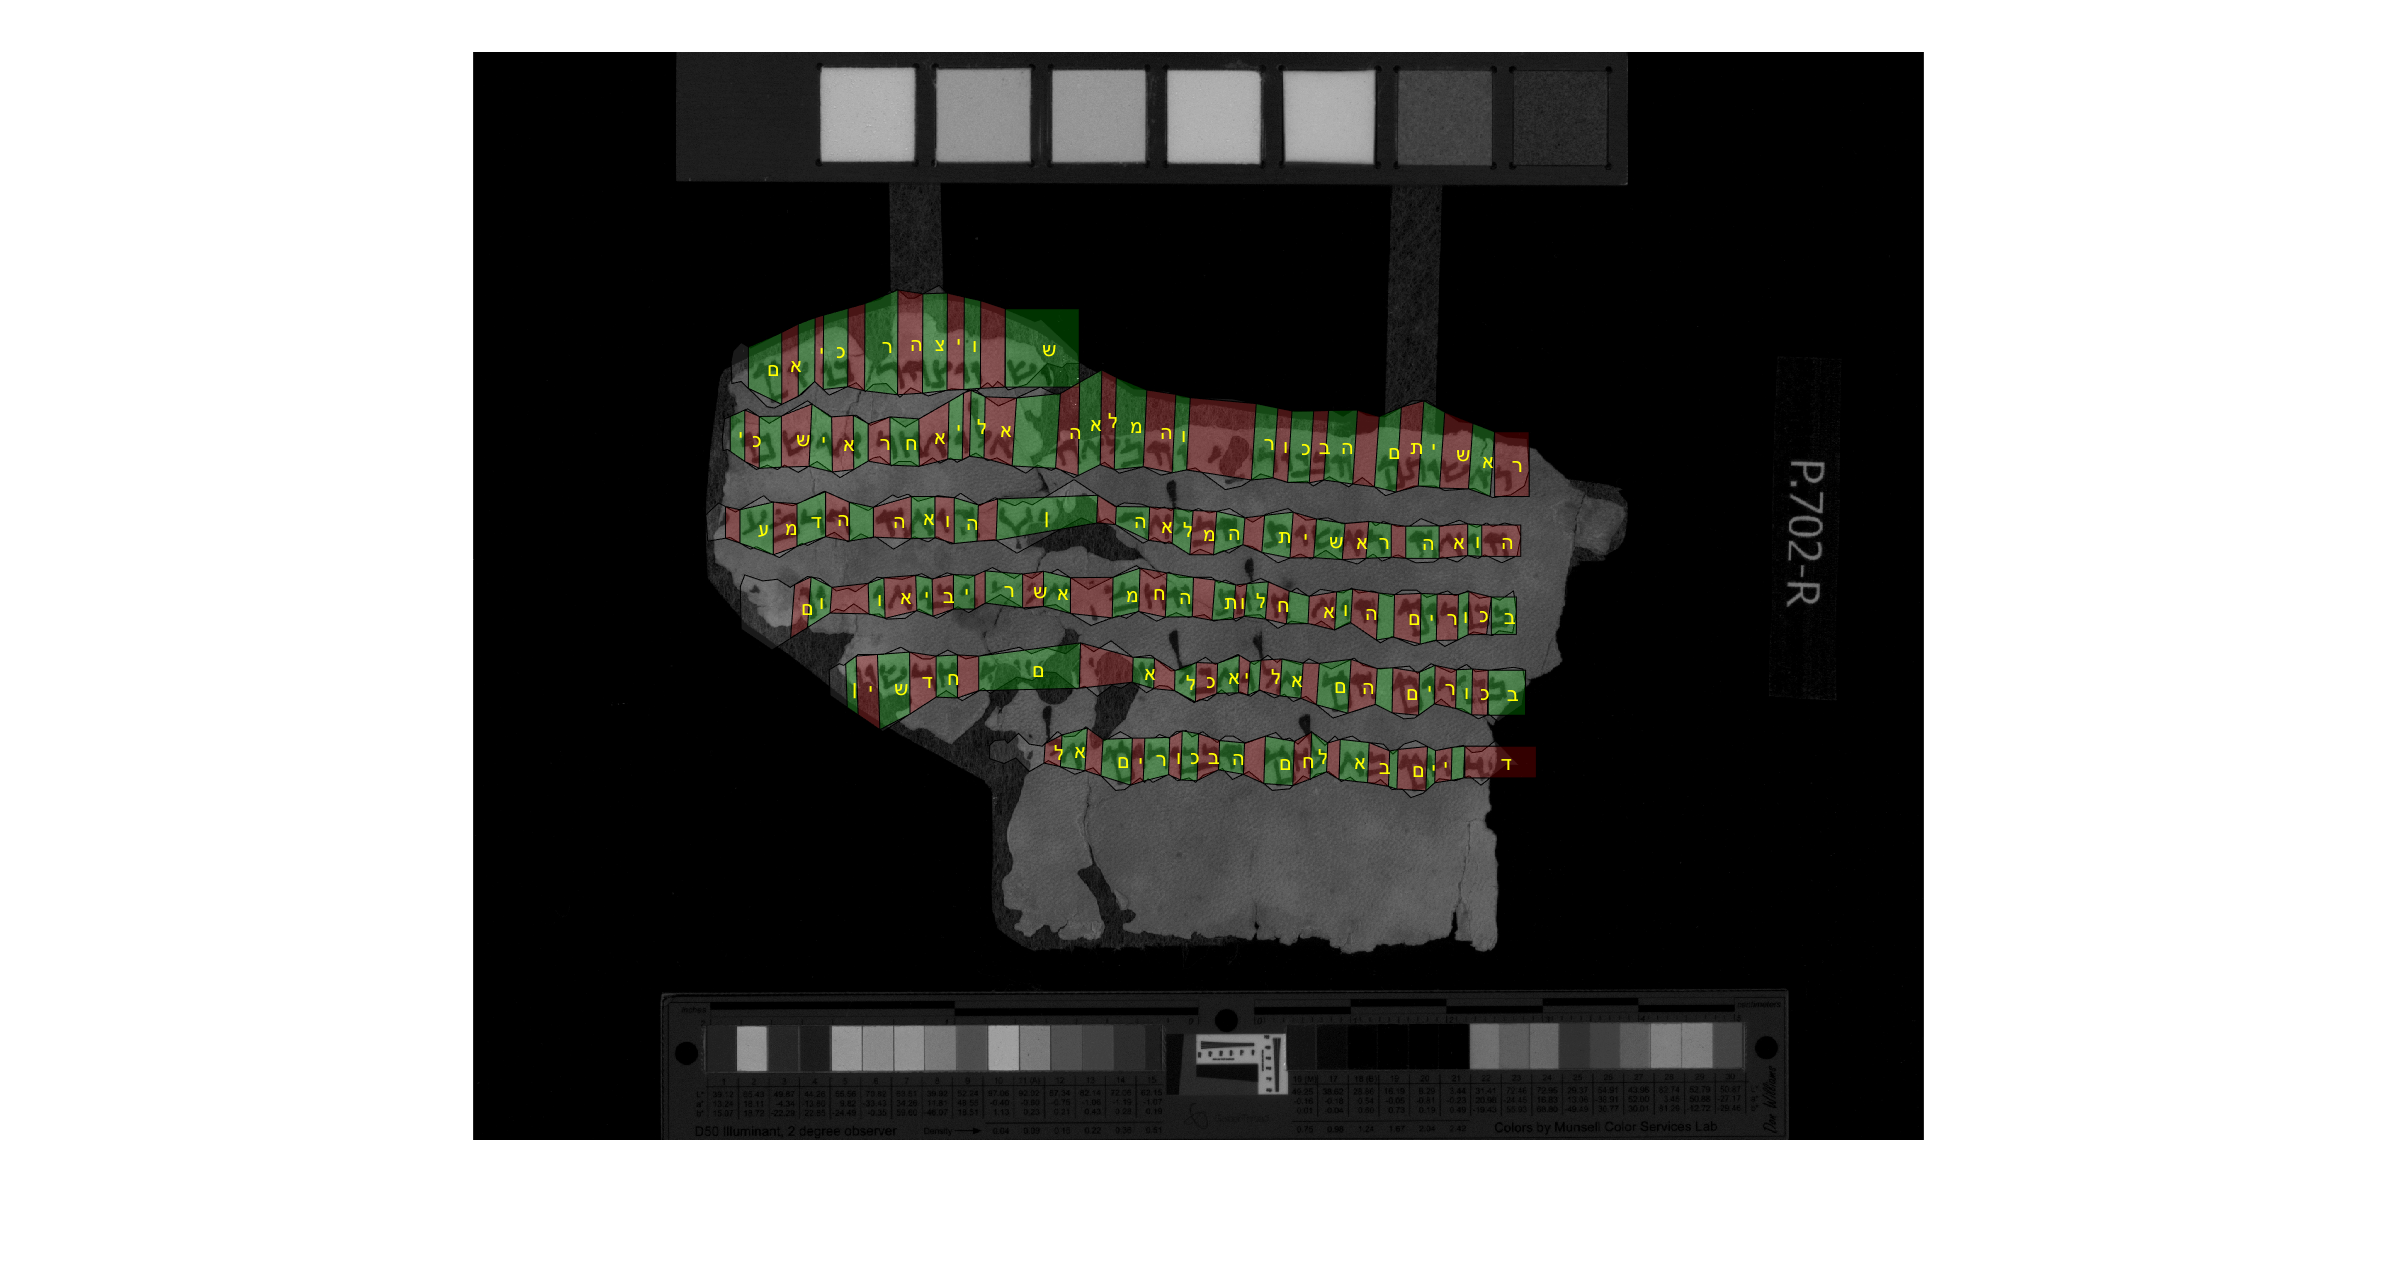
\includegraphics[width=1.0\linewidth]{images/P702-Fg010-R-C01-R01-D12092012-T111025-LR924_012_F_rewrite._reordered_with_text._page.png}
%\label{fig:regularAlignment} \end{subfigure} \begin{subfigure}{0.48\textwidth}
%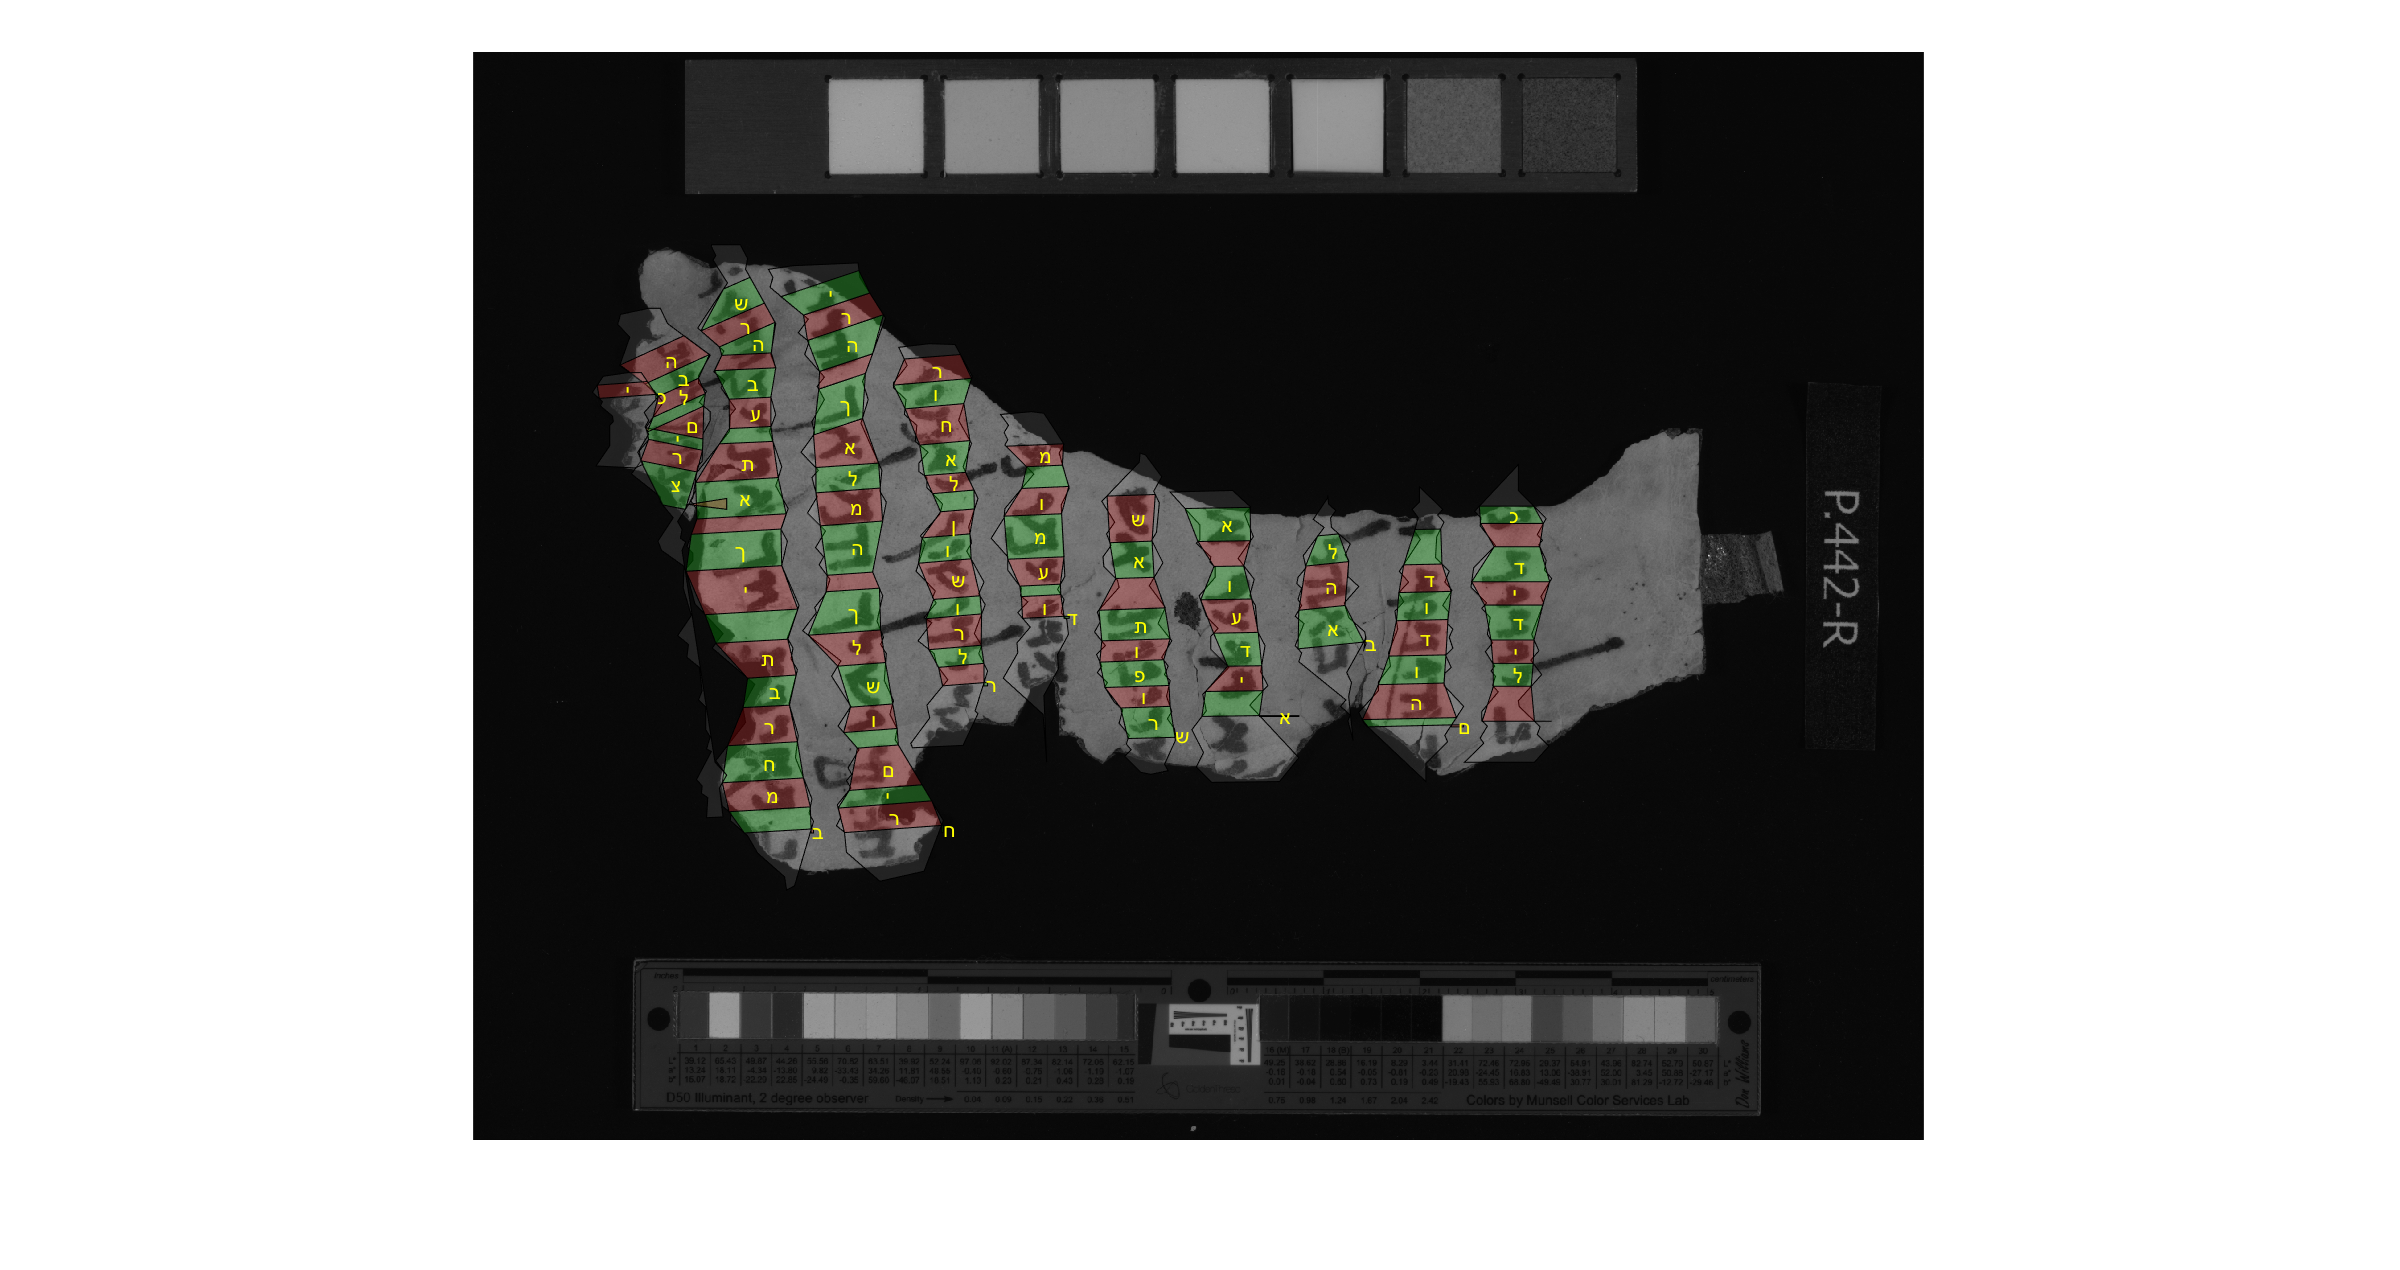
\includegraphics[width=1.0\linewidth]{images/P442-Fg001-R-C01-R01-D01092013-T114646-LR924_012_rewrite._reordered_with_text._page.png}
%\label{fig:rotatedAlignment} \end{subfigure}
%
%\caption{Transcription alignment example.}

%\label{fig:align} \end{figure*}

To evaluate the various transcription alignment algorithms' performance, we
compared the automatic alignment with the bounding boxes from a set consisting
of 1278 letters that had been expertly segmented by hand using the Scripta
Qumranica Electronica website.  We denote a glyph as correctly aligned if the
correct glyph in the manuscript is the closest one to the computed glyph
location.  To measure the distance between letters, we use Euclidean distance
between the centers of the bounding boxes of the glyphs.

% Tables of success rate for alignment.  Optical flow - accuracy without
% anchors - 48.1\% .  Accuracy with added anchors of interword spaces - 74\%.
% OCR derived alignment accuracy - $\mathbf{90.3\%}$. 

\begin{center} \begin{tabular}{ |p{5cm}||c|  } \hline
	\multicolumn{2}{|c|}{\textbf{Transcription alignment accuracy}} \\
	\hline Method& Accuracy\\ \hline Optical flow without anchors&48.1\%\\
	Optical flow with added anchors&74.0\%\\ OCR derived alignment&
	$\mathbf{90.3\%}$\\ \hline \end{tabular} \end{center}

To further examine the performance of our leading transcription alignment
method, we measured the proportion of the intersection area of the bounding
polygon of the glyph of the OCR system and the human annotated ground truth: 

% OCR and GT polygons overlap percentages (out of GT polygon) - 81\% mean,
% 87.1\% median, 20.5\% standard deviation.

\begin{center} \begin{tabular}{ |p{3cm}||c|c| } \hline
	\multicolumn{3}{|c|}{\textbf{OCR bounding boxes overlap with ground
	truth}} \\ \hline Statistic&Area& Area percentage\\ \hline
	Average&31.0&81.0\%\\ Median&23.8&87.1\%\\ Standard
	deviation&30.8&20.5\%\\ \hline \end{tabular} \end{center}

As can be seen, the accuracy of the OCR based transcription alignment method is
the highest among the methods we've used, and the intersection of the
recognized bounding polygon with the original glyph bounding box is high as
well.  An alignment example is displayed in Fig.~\ref{fig:align}.  The
interword space in line 2, for instance, has been well detected and shows that
our alignment method provides excellent results on the word level.
Fig.~\ref{fig:alignedGlyphs} shows aligned glyphs of a single line compared to
the ground truth.  Finally, the ground truth allows for overlapping glyph
bounding boxes, a feature impossible for the current and all other known
algorithms.

An analysis of the errors shows that the results can be further improved as
some letters and some positions quite consistently reveal a higher error
proportion.  The letter lamed, which has a high ascender, is frequently cut
below its top by the seamcarve algorithm, often because of the deterioration of
the writing material.  Similarly final mem has a long descender and can be cut
too high.  Finally, the seamcarve algorithm uses the neighboring lines to limit
the height of rows.  This is impossible for the upper boundary of the top and
the lower boundary of the bottom rows.  For all of these problems with $y$
coordinates, obvious solutions tailored to the type of script and material are
available.  Otherwise, the method use should be able to be applied to other
sequential scripts.

% 0,clip,width=.49\linewidth]{images/P702-Fg010-R-C01-R01-D12092012-T111025-LR924_012_F_rewrite._reordered_with_text._page.png}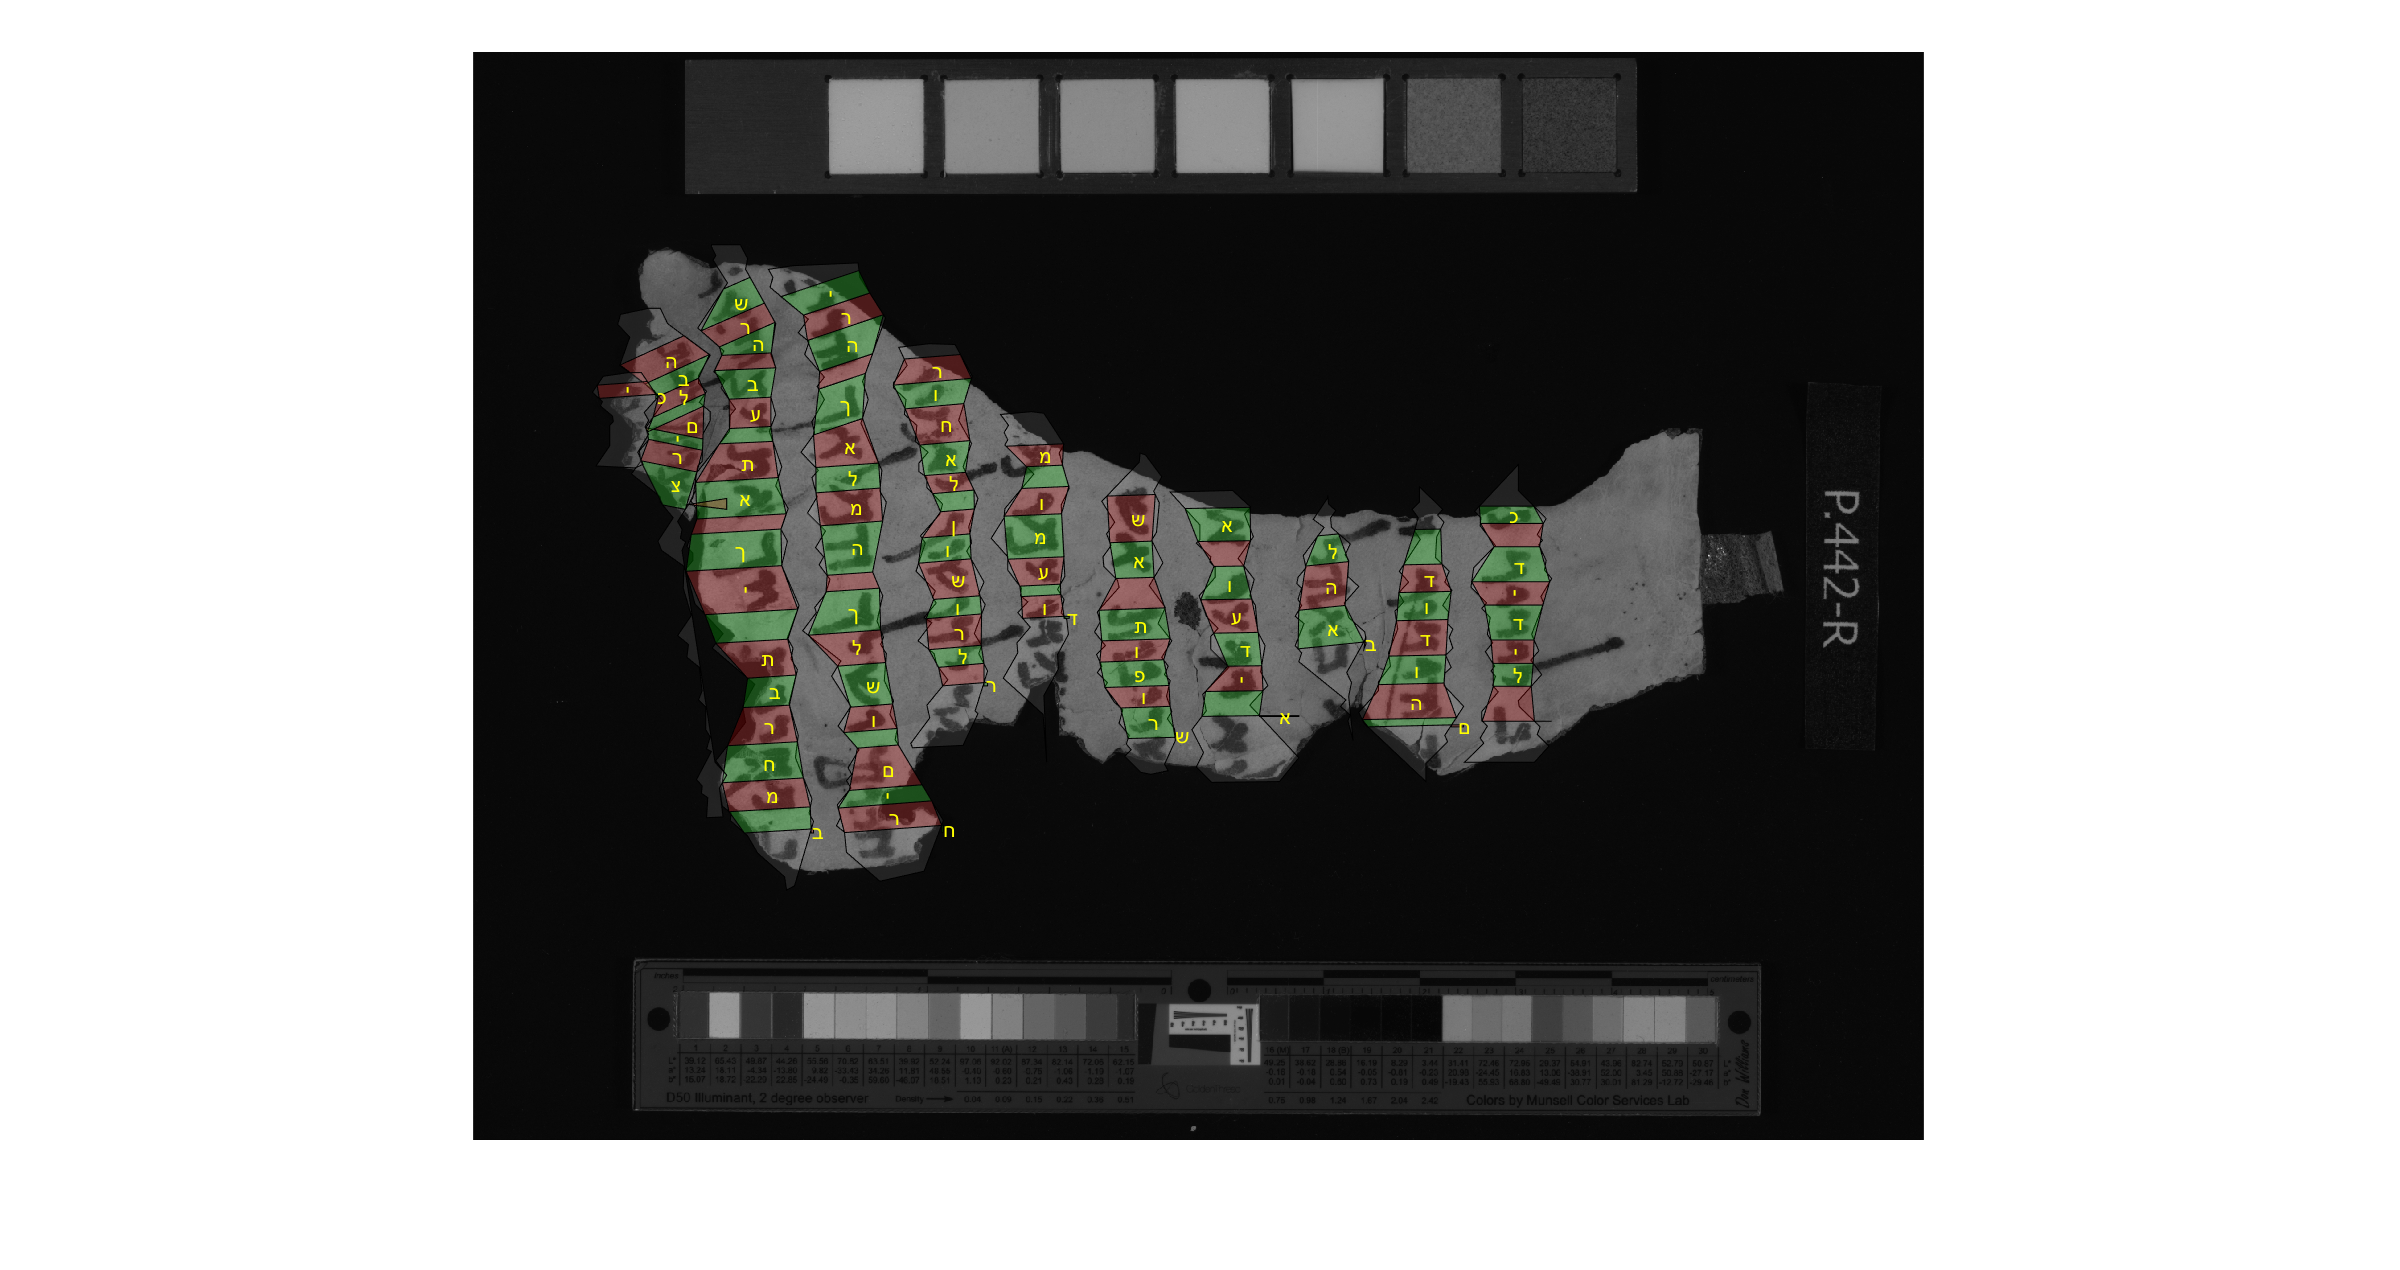
\includegraphics[trim=200
% 0 200
% 0,clip,width=.49\linewidth]{images/P442-Fg001-R-C01-R01-D01092013-T114646-LR924_012_rewrite._reordered_with_text._page.png}
% \caption{Two examples of alignment, the left upright, and the right, rotated
% 90{\degree}.}\label{fig:align} \end{figure}

\section{Discussion}

We have put together an end-to-end automated pipeline for processing images and
transcriptions of the very fragmentary Dead Sea Scroll manuscripts.  Despite
the many difficulties posed by the often seriously degraded material, the
quality of segmentation and character recognition were sufficient to allow a
glyph-by-glyph alignment of existing transcriptions to the new, high-quality
images.  The successful identification of fragments based on automatic
transcriptions holds promise of helping to identify some of the remaining
unidentified fragments of the image database with their counterparts in the
text database.  Each of the stages of the pipeline, viz.\@ (A) baseline layout
analysis of the fragment and (B) segmentation into line polygons, (C) rough
automated transcription of the text in each of the fragment lines, and (D)
alignment of the rough automatic transcription to the scholarly transcriptions
to the image of the fragment, can be improved further.

The successful automated alignment of transcriptions to images will allow a
textual layer to be added to the IAA images.  This means that scholars and
laypersons alike will be able to enter search terms and retrieve images
containing them.  It will also supply additional training data for improved
character recognition and future paleographical analyses.

\section*{Acknowledgments} This research was supported in part by Grant BE
5916/1-1 KR 1473/8-1 from the Deutsch-Israelische Projektkooperation (DIP) and
by Grant Agreement No. 871127 from the European Union’s Horizon 2020 Research
and Innovation Programme.  It was made possible thanks to images taken by Shay
Halevi and provided by the Leon Levy Dead Sea Scrolls Digital Library of the
Israel Antiquities Authority, all rights reserved.  We thank the SQE project
members, especially Oren Ableman, Adiel Ben-Shalom, and Lior Wolf.
